
\begin{obs}
Si en  (\ref{def:FuncMate1})  cambiemos  $A \subseteq \mathbb{R}$ y $B\subseteq \mathbb{R}$ por $A \subseteq \mathbb{R}^{n}$ y $B \subseteq \mathbb{R}^{m}$  obtenemos de manera analoga la siguiente definici\'on.    
\end{obs}





\begin{definition} \textbf{Campos.}
  Un \textit{campo} es una funci\'on   $\campoVec{F}:A\subseteq \mathbb{R}^n \rightarrow B \subseteq \mathbb{R}^m.$    Si $m=1$ lo llamaremos  \textit{ campo escalar }  y  si  $m\geq 2$ lo llamaremos   \textit{ campo vectorial}. Al igual que en (\ref{def:FuncMate1}), a los conjuntos $A$ y $B$  se los llama, respectivamente, \textit{dominio}  y \textit{codominio} del campo $\campoVec{F}$ y  la notaci\'on usual para los mismos  es  $A=\text{Dom}( \campoVec{F})$ y $B=\text{Cod}( \campoVec{F})$.   
  \end{definition}
  
\textbf{Notaci\'on: } En general, la notaci\'on usual  para campos escalares es  con letras imprentas minúsculas y para  los campos vectorials es con letra imprenta mayúscula y negrita. A lo largo del documento mantendremos esta notación. 
  
  \begin{definition} {\textbf{Componentes de un campo vectorial.}}
  Sea   $\campoVec{F}:A\subseteq \mathbb{R}^n \rightarrow B \subseteq \mathbb{R}^m$   un \textit{campo vectorial}, dado $\vect{x}_0 \in A$ se puede pensar a  $\mathbf{F}(\vect{x}_0)$   como la evaluación de $m$ campos escalares en $\vect{x}_0$, 
    es decir,
    \begin{equation*}
        \campoVec{F}(\vect{x}_0)=\big( f_1(\vect{x}_0),..., f_m(\vect{x}_0) \big).
    \end{equation*}
  Para $1 \leq i \leq n$,  el campo escalar $f_i: A\subseteq \mathbb{R}^n \rightarrow  \mathbb{R}$ se llama la \textit{i-\'esima componente} de $\campoVec{F}.$
 \end{definition}
  
  
  \begin{definition}{\textbf{Conjunto Imagen.}}
    Sea  $\campoVec{F}:A\subseteq \mathbb{R}^n \rightarrow B \subseteq \mathbb{R}^m$, se define el \textit{conjunto imagen} de $\mathbf{F}$, y se denota por $ \operatorname{Img}(\mathbf{F})$, a 
    \begin{equation*}
        \operatorname{Img}(\campoVec{F})=\{\mathbf{y}\in\mathbb{R}^m: \mathbf{F}(\mathbf{x})=\mathbf{y}, \mathbf{x} \in A\}.
    \end{equation*}
  \end{definition}
  
  
 
\begin{example} \label{ej:campoEscalar}
La función $d \colon \mathbb{R}^3 \to \mathbb{R}$ definida por $d(x,y,z) = \sqrt{x^2+y^2+z^2}$ es un campo escalar. En este caso, $\operatorname{Dom}(d) = \mathbb{R}^{3}$, $\operatorname{Cod}(d) = \mathbb{R}$ y $\operatorname{Img}(d) = \mathbb{R}_{\geq 0}$.  Para cada  punto $(x,y,z)$  el campo $d$ devuelve la distancia eucl\'idea de dicho punto  al $(0,0,0)$. Por ejemplo,  tomemos el punto $(1,2,2) \in \mathbb{R}^{3}$ entones $\text{d}(1,2,2)= 3$ es la distancia  eucl\'idea  del punto $(1,2,2)$ al punto $(0,0,0).$
Esta relación también se puede visualizar como:
\end{example}
  

\begin{figure}[H]
\centering
\begin{tikzpicture}[scale=1]

% --- Espacio R^3 (dominio) a la izquierda ---
\begin{axis}[
    at={(0,0)},
    anchor=center,        
    width=6cm, height=6cm,
    view={120}{30},
    axis lines=middle,
    axis line style={black!70},
    label style={black!70},
    ticks=none,
    xlabel={$x$}, ylabel={$y$}, zlabel={$z$},
    xmin=0, xmax=3,
    ymin=0, ymax=3,
    zmin=0, zmax=3,
]
% Punto (1,2,2) en R^3
\addplot3[only marks, mark=*, red] coordinates {(1,2,2)};
\node at (axis cs:1,2,2.5) {\textcolor{red}{$(1,2,2)$}}; 
\end{axis}

% --- Título dominio ---
\node at (0,3.3) {Dominio};


% --- Espacio R (codominio) a la derecha como recta numérica ---
% Se usa la punta stealth-stealth para indicar recta infinita en ambos lados
\draw[stealth-stealth, thick, black!70] (5.5,0) -- (10.5,0);

% Título del codominio arriba de la recta
\node at (8,0.5) {Codominio};

% Marca del Origen (0) en la recta numérica
\draw[thick, black!70] (6, -0.1) -- (6, 0.1);
\node at (6, -0.4) {\small $0$};

% --- Pintar la Semirrecta en Azul: Imagen del conjunto [0, +infinito) ---
% Comienza con un corchete en (6,0) y se extiende hasta la punta de la flecha en (10.5,0)
\draw[blue, ultra thick, -stealth] (6,0) -- (10.5,0);

% Corchete izquierdo del intervalo cerrado en el cero
\node[blue] at (6,0) {\textbf{[}};

% Punto Imagen particular d(1,2,2) = 3 (destacado encima de la semirrecta)
\filldraw[blue] (9,0) circle (2pt);
\node at (9,0.4) {\textcolor{blue}{$3$}};


% --- Título general sobre el bloque de la derecha ---
\node at (8,3.3) {Codominio};


% --- Flecha curvada entre los puntos ---
\draw[->, thick, black] (1.8,0.5) .. controls (3.5,2.0) and (4.8,1.7) .. (5.4,0.3);
\node at (3.65,1.8) {\Large $d$};

\end{tikzpicture}
\caption{Visualización de $(1,2,2)$, su imagen $d(1,2,2)=3$ y el conjunto imagen $\operatorname{Img}(d) = \mathbb{R}_{\geq 0}$ resaltado en azul.}
\label{fig:visualizacion_campo_escalar_con_semirrecta}
\end{figure}


\begin{tarea} Hallar todos los puntos $(x,y,z) \in \mathbb{R}^{3}$ tales que  $d(x,y,z)=3$ y dibujarlos. 
\end{tarea}  





\begin{example}
Probar que la transformación lineal $\campoVec{T} \colon \mathbb{R}^2 \to \mathbb{R}^3$ es efectivamente una transformación lineal y calcular su imagen,  siendo $$\campoVec{T}(x,y) = (x+y, x-y, x+y)$$ 
\end{example}

Se deja a cargo del lector probar que $\campoVec{T}$ verifica la \autoref{def:TL}. Para encontrar su imagen, basta con escribir:
\begin{align*}
\campoVec{T}(u_1, u_2) &= (u_1+u_2, u_1-u_2, u_1+u_2) \\
&= (u_1, u_1, u_1) + (u_2, -u_2, u_2) \\
&= u_1(1,1,1) + u_2(1,-1,1), \quad \text{con } u_1, u_2 \in \mathbb{R}.
\end{align*}
Así, la imagen resulta el siguiente plano en $\mathbb{R}^3$ (ver \autoref{def:planoR3}):
\begin{equation*}
\operatorname{Img}(\campoVec{T}) = \{ \vect{x} \in \mathbb{R}^3 \mid \vect{x} = u_1(1,1,1) + u_2(1,-1,1), \; u_1, u_2 \in \mathbb{R} \}.
\end{equation*}
Otra manera equivalente de representar dicho plano es mediante la ecuación:
\[ z = x.\]Finalmente, se puede representar gráficamente el dominio y el codominio.


\begin{figure}[H]
\centering
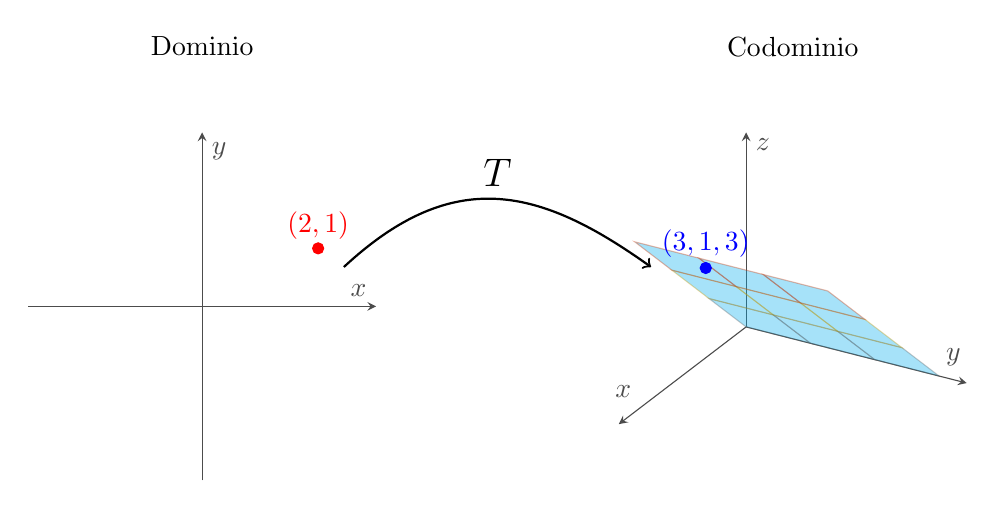
\begin{tikzpicture}[scale=1]

% --- Espacio R^2 (dominio) a la izquierda (Cuatro Cuadrantes) ---
\begin{axis}[
    at={(0,0)},
    anchor=center,        % Cambiado a center para estabilidad geométrica
    width=6cm, height=6cm,
    axis lines=middle,
    axis line style={black!70},
    label style={black!70},
    ticks=none,
    xlabel={$x$}, ylabel={$y$},
    xmin=-3, xmax=3,      
    ymin=-3, ymax=3,      
]
% Punto (2,1) en R^2
\addplot[only marks, mark=*, red] coordinates {(2,1)};
\node at (axis cs:2,1.4) {\textcolor{red}{$(2,1)$}};
\end{axis}

% --- Título dominio ---
\node at (0,3.3) {Dominio};


% --- Espacio R^3 (codominio) a la derecha ---
\begin{axis}[
    at={(7.5cm,0)},       % Alineado horizontalmente a 7.5cm y verticalmente en 0
    anchor=center,        % Anclado al centro para una alineación vertical perfecta
    width=6cm, height=6cm,
    view={120}{30},
    axis lines=middle,
    axis line style={black!70},
    label style={black!70},
    ticks=none,
    xlabel={$x$}, ylabel={$y$}, zlabel={$z$},
    xmin=0, xmax=4,
    ymin=0, ymax=4,
    zmin=0, zmax=4,
]
% --- Dibujo del Plano z = x (Imagen real de T) ---
\addplot3[
    surf,
    fill=cyan,           
    opacity=0.35,        
    draw=cyan!60!black,  
    domain=0:3.5,        
    domain y=0:3.5,      
    samples=4,           
] {x};

% Punto (3,1,3) en R^3
\addplot3[only marks, mark=*, blue] coordinates {(3,1,3)};
\node at (axis cs:3,1,3.5) {\textcolor{blue}{$(3,1,3)$}};
\end{axis}

% --- Título codominio ---
% Reubicado de forma simétrica sobre el eje del codominio
\node at (7.5,3.3) {Codominio};


% --- Flecha curvada entre los puntos (Perfectamente balanceada) ---
% Ahora usa coordenadas relativas al centro de cada bloque, garantizando simetría
\draw[->, thick, black] (1.8,0.5) .. controls (3.2,1.8) and (4.3,1.5) .. (5.7,0.5);
\node at (3.75,1.7) {\Large$\campoVec{T}$};

\end{tikzpicture}
\caption{Visualización de $(2,1)$, su imagen $\campoVec{T}(2,1) = (3,1,3)$ y el plano $z = x$.}
\label{fig:visualizacion_T_con_plano_simetrico}
\end{figure}



       \begin{example}  \label{ej:campoVectorial}
        La función $\mathbf{F}:\mathbb{R}^2 \rightarrow \mathbb{R}^3 \;|\; \mathbf{F}(x,y) = (x+y,x-y,xy)$ es un campo vectorial. 
        En este caso, su dominio es $\mathbb{R}^2 $ y su codominio $\mathbb{R}^3 $.
        
      La imágen de $\mathbf{F}$ se puede hallar con el siguiente planteo:
        \begin{equation*}
          \mathbf{F}(x,y) = (x+y,x-y,xy) = (u,v,w)  .
        \end{equation*}
        Luego, resolviendo el sistema de ecuaciones resultante, se llega a la ecuación
        \begin{equation*}
          w = \frac{u^2}{4}-\frac{v^2}{4},
        \end{equation*} y, por lo tanto, queda 
         \begin{equation}\label{imagF}
          \text{Img}(\mathbf{F})=\left\{ (u,v,w)\in\R^3 \:\Big|\: w=\frac{u^2}{4}-\frac{v^2}{4} \right\}
        \end{equation}  la cual describe  un paraboloide hiperbólico en $\mathbb{R}^3.$ 
       
Visualicemos  la relaci\'on entre  el dominio y la imagen de campo vectorial $\mathbf{F}$ con un caso particular, para ello tomemos el punto $(1,1) \in \mathbb{R}^{2},$  luego $ \mathbf{F}(1,1)=(2,0,1) \in  \text{Img}(\mathbf{F})$
 
 \begin{figure}[H]
  \begin{center}
    \begin{tikzpicture}

      % Plano 2D a la izquierda
      \begin{axis}[
        at={(0,0)},
        anchor=origin,
        axis lines=middle,
        axis line style={black!70},
        label style={black!70},
        ticks=none,
        xlabel={$x$}, ylabel={$y$},
        xmin=-1, xmax=3,
        ymin=-1, ymax=3,
        width=6cm,
        height=6cm,
        title={Dominio}
      ]
        % Punto (1,1)
        \addplot[only marks, mark=*, red] coordinates {(1,1)};
        \node at (axis cs:1.3,0.6) {\textcolor{red}{$(1,1)$}};
      \end{axis}
    
      % Espacio 3D a la derecha, alineado
      \begin{axis}[
        at={(7cm,0.5cm)},
        anchor=origin,
        view={130}{30},
        axis lines=middle,
        axis line style={black!70},
        label style={black!70},
        ticks=none,
        xlabel={$x$}, ylabel={$y$}, zlabel={$z$},
        xmin=-1, xmax=4,
        ymin=-1, ymax=2.5,
        zmin=-1, zmax=3,
        width=7cm,
        height=7cm,
        title={Codominio}
      ]
        % Punto imagen (2,0,1)
        \addplot3[only marks, mark=*, blue] coordinates {(2,0,1)};
        \node at (axis cs:3.5,0.2,1.2) {\textcolor{blue}{$(2,0,1)$}};
      \end{axis}
    
      % Flecha curva más simple
      % Puntos de origen y destino
      \coordinate (A) at (1.3,1.4);
      \coordinate (B) at (3,0);
    
      % Dibujo del arco como flecha
      \draw[->, thick]
        (A) arc[start angle=120, end angle=50, radius=4cm];
    
      % Etiqueta
      \node at (4,1.5) {$\mathbf{T}$};
    \end{tikzpicture}
   \caption {Visualización de $(1,1)$ y $\mathbf{F}(1,1)=(2,0,1)$}
   \end{center}
 \end{figure}
\end{example} 

\begin{tarea} Graficar   $ \text{Img}(\campoVec{F})  \: (\ref{imagF}).$
\end{tarea}

    
